\documentclass[a4paper]{jpconf}
\bibliographystyle{iopart-num}
\usepackage{silence}
\WarningsOff[caption]
\usepackage{graphicx}
\usepackage{hyperref}
\usepackage{cleveref}
\usepackage{amsmath}
\usepackage{fix-cm}
\usepackage[hypcap=false, font=small,labelfont=bf]{caption}
\begin{document}
\crefname{equation}{Equation}{Equations}
\crefname{chapter}{Chapter}{Chapters}
\crefname{section}{Section}{Sections}
\crefname{appendix}{Appendix}{Appendices}
\crefname{enumi}{Item}{Items}
\crefname{footnote}{Footnote}{Footnotes}
\crefname{figure}{Figure}{Figures}
\crefname{table}{Table}{Tables}
\crefname{theorem}{Theorem}{Theorems}
\crefname{lemma}{Lemma}{Lemmas}
\crefname{corollary}{Corollary}{Corollaries}
\crefname{proposition}{Proposition}{Propositions}
\crefname{definition}{Definition}{Definitions}
\crefname{result}{Result}{Results}
\crefname{example}{Example}{Examples}
\crefname{remark}{Remark}{Remarks}
\crefname{note}{Note}{Notes}

\title{Numerical simulation of turbulent flow in a cyclonic separator}

\author{Dmitry Bogdanov and Sergey Poniaev}

\address{Division of Plasma Physics, Atomic Physics and Astrophysics, Ioffe Physical Technical Institute, 26 Polytekhnicheskaya, St Petersburg 194021, Russian Federation}

\ead{\href{mailto:dimyriy.bogdanov@gmail.com}{dimyriy.bogdanov@gmail.com}}

\begin{abstract}
Abstract. Numerical simulation of a turbulent flow of air with dispersed particles through 
a cyclonic separator is presented. Because of a high streamline curvature in the separator it 
is difficult to simulate the flow by using the conventional turbulent models. In this work the 
curvature correction term was included into the $k-\omega-SST$ turbulence model implemented in 
the OpenFOAM{\textregistered} software. Experimental data and results of numerical simulation by the
commercial ANSYS Fluent{\textregistered} solver for a turbulent flow in a U-duct were used to validate the 
model. The numerical simulation of the flow in the cyclonic separator demonstrates that the 
implemented turbulence model successfully predicts the cyclonic separator efficiency.
\end{abstract}
\section{Introduction}
Cyclonic separators are widely used for dispersed phase separation from the gas \cite{instructions} . One of 
their important parameters is the efficiency which is the ratio between the number of filtered 
particles and the total number of particles injected into a cyclonic separator. However, it is 
extremely difficult to predict the separator efficiency by using numerical simulation of the 
turbulent flow because conventional eddy-viscosity models cannot adequately describe the 
flow \cite{ShurSpallart} because of a high streamline curvature and, more specifically, inadequate calculation  of the turbulence kinetic energy production. The kinetic energy production can be corrected by using the Shur-Spalart curvature correction function for the Spalart-Allmaras turbulence model reformulated in \cite{Smirnov} in terms of the $k-\omega-SST$ turbulence model.

\section{Cyclonic separator model}
A typical scheme of the air flow in cyclone is presented in \cref{fig:physicalModel} \cite{instructions}. The air with dispersed particles enters the cyclone through an air inlet. Under the centrifugal forces heavy particles move to the boundary layer on a sidewall. move to the boundary layer on a sidewall. The influence of the air flow on the particles which have moved to the boundary layer is relatively weak as compared with the influence of the gravity force and hence particles fall to the dust chamber. The air leaves the cyclone through an air outlet.
\section{SST with curvature correction model formulation}
\label{sec:model}
As stated above, a correction of the SST turbulence model is needed because of a high streamline curvature. In this paper the correction function \eqref{eq:1} suggested in \cite{ShurSpallart} is used as a multiplier of the production term in the Spalart-Allmaras eddy viscosity transport equation. In \cite{Smirnov}, it is suggested that this function be used with respect to the SST model as follows

\begin{equation}
\label{eq:1}
f_{rotation} = (1+c_{r_1}) \frac{2r^*}{1+r^*} [1-c_{r_3}\tan^{-1}(c_{r_2}\tilde{r})] -c_{r_1}
\end{equation}

\begin{figure}[h]
\begin{minipage}{14pc}
\includegraphics[width=8pc]{flowScheme1.png}\hspace{6pc}
\caption{\label{fig:physicalModel} Scheme of the air flow inside cyclonic separator.}
\end{minipage}
\begin{minipage}{20pc}
Article \cite{Smirnov} suggests to use this function as follows in respect to the SST model.

\begin{equation}
\label{eq:2}
\frac{\partial (\rho k)}{\partial t} + \frac{\partial (\rho u_j k)}{\partial x_j} = P_k f_{r_1} - \beta^* \rho k \omega + \frac{\partial}{\partial x_j} \left[ \mu_{eff}\frac{\partial k}{\partial x_j} \right]
\end{equation}

\begin{equation}
\begin{split}
\frac{\partial (\rho \omega)}{\partial t} + \frac{\partial (\rho u_j \omega)}{\partial x_j} = \alpha \frac{\rho P_k}{\mu_t}f_{r_1}  - \beta \rho \omega^2 +\\
+ 2\left(1-F_1\right()\frac{\rho \sigma_{\omega_2}}{\omega}\frac{\partial k}{\partial x_j}\frac{\partial \omega}{\partial x_j} + \frac{\partial}{\partial x_j} \left[ \mu_{eff}\frac{\partial \omega}{\partial x_j} \right]
\end{split}
\end{equation}

\begin{equation}
f_{r_1} = \max\left[ \min(f_{rotation}, 1.25), 0 \right]
\end{equation}

\begin{equation}
r^*=\frac{S}{\Omega}, \quad \mu_{eff}=\mu_t + \sigma_{k/\omega}\mu_t
\end{equation}

\end{minipage}
\end{figure}
\begin{equation}
\tilde{r} = 2\Omega_{ik}S_{jk}\left[ \frac{DS_{ij}}{Dt} + \left( \varepsilon_{imn}S_{jn} + \varepsilon_{jmn}S_{in} \right)\Omega^{rot}_m \right]\frac{1}{\Omega D^3}
\end{equation}

 \begin{equation}
 S_{ij} = \frac{1}{2}\left( \frac{\partial u_i}{\partial x_j} + \frac{\partial u_j}{\partial x_i} \right)
 \end{equation}

\begin{equation}
\Omega_{ij} = \frac{1}{2}\left( \left( \frac{\partial u_i}{\partial x_j} - \frac{\partial u_j}{\partial x_i}  \right) +2\varepsilon_{mji} \Omega^{rot}_m \right)
\end{equation}

\begin{equation}
S^2 = 2S_{ij}S_{ij}, \quad 
\Omega^2 = 2\Omega_{ij}\Omega_{ij}
\end{equation}

\begin{equation}
D^2 = \max(S^2, 0.09\omega^2)
\end{equation}

$$
c_{r_1} = 1.0, \quad c_{r_2} = 2.0, \quad c_{r_3} = 1.0
$$
 where $u_i$ represents velocity components, $\rho$ - gas density, $k$ is for turbulence kinetic energy, $\omega$ is for specific dissipation rate, $S_{ij}$ - strain rate tensor, $\Omega_{ij}$ - vorticity rate, $P_k$ - production term for SST model, $f_{r_1}$ - correction function for the SST model, $f_{rotation}$ - correction function for the Spalart-Almaras model, $\mu_{t}$ - turbulence eddy viscosity and $DS_{ij}/Dt$ represents the components of the Lagrangian derivative of the strain rate tensor. $\alpha$, $beta$, $\beta^*$, $C$ - standard SST model constants, $c_{r_1}$, $c_{r_2}$, $c_{r_3}$ - SST-CC model constants, $F_1$ - additional function from standard SST model \cite{Menter}.

\section{Model validation}

The turbulence model described in \cref{sec:model} was implemented by using the OpenFOAM{\textregistered} mathematical library. Model validation was performed by using the Monson \cite{Monson} experimental data for a turbulent flow in a U-duct and numerical simulation in ANSYS Fluent{\textregistered}. Geometric and flow parameters for the U-duct are listed in \cref{table:1}. The flow scheme is presented in \cref{fig:uDuctScheme}.
The inlet profile used as the inlet boundary condition was obtained from preliminary 
computations of the turbulent flow in a plane channel, because in the Monson experiment \cite{Monson} the 
flow was assumed to be fully developed in the inlet section. Numerical simulation of the flow 
was performed by using standard SST and SST with the curvature correction term (SST-CC) in 
both solvers.

Results of numerical simulation for velocity projections $U_x$ and $U_y$ in different cross-sections of the channel are shown in \cref{fig:x0up,fig:x0down,fig:y0,fig:x1down}. \cref{fig:x0up} shows velocity profiles before U-turn. Because the flow curvature in this cross section is negligibly small, both models (SST and SST-CC) in both solvers give the same results which are in very good agreement with experimental data. \cref{fig:y0}  shows velocity  profiles at the center of the U-turn. As one can see from \cref{fig:y0}, the OpenFOAM{\textregistered} results are closer to the experimental values, and the results with the SST-CC model are better than those with the SST model. \cref{fig:x0down} shows velocity profiles immediately after U-turn. It is evident that SST-CC is much better than SST for both solvers. OpenFOAM{\textregistered} results are better on the inner wall of the cnahhel and worse on the outer wall as compared with Fluent{\textregistered}. \cref{fig:x1down} shows velocity profiles in the cross-section at the distance of the one caliber after the U-turn. The flow curvature is small here, so the difference between SST-CC and SST is insignificant and, like in the previous cross-section, the OpenFOAM{\textregistered} results are better on the inner wall of the channel and worse on the outer wall as compares with Fluent{\textregistered}.

\begin{figure}[h]
\begin{minipage}{18pc}
\begin{center}
\captionof{table}{\label{table:1} Geometric and flow parameters for air flow in U-duct.}
\begin{tabular}{{r}{l}}
\br
Channel height, $H$ & $3.81cm$\cr
Channel length, $L$ & $10H$\cr
Inner radius, $R_i$ & $1.91cm$\cr
Outer radius, $R_o$ & $5.72cm$\cr
Av. velocity at inlet $U_{in}$ & $30.1m/s$\cr
Av. temperature at inlet, $T_{in}$ & $264K$\cr
Pressure at outlet, $p_{out}$ & $1.15atm$\cr
Reynolds number, Re & $~10^5$\cr
\end{tabular}
\end{center}
\end{minipage}
\begin{minipage}{19pc}
\begin{center}
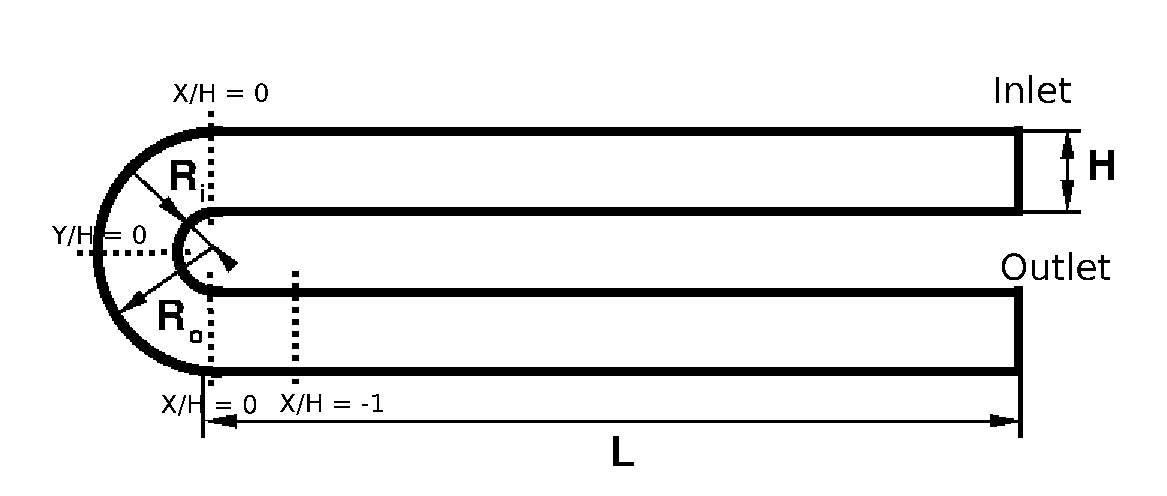
\includegraphics[width=19pc]{UDuct.eps}
\hspace{1em}\captionof{figure}{\label{fig:uDuctScheme} Scheme of flow in U-duct for the Monson experiment simulation}
\end{center}
\end{minipage}
\end{figure}
\begin{figure}[ht]
	\begin{minipage}{0.475\linewidth}
		\includegraphics[scale=0.33]{xh0up}
		\caption{$U_x$ velocity component distribution in $x/H=0$ cross-section (top channel).}
		\label{fig:x0up}
	\end{minipage}
	\hspace{0.5em}
	\begin{minipage}{0.475\linewidth}
		\includegraphics[scale=0.33]{yh0}
		\caption{$U_y$ velocity component distribution in $y/H=0$ cross-section.}
		\label{fig:y0}
	\end{minipage}
\end{figure}
\begin{figure}[ht]
	\vspace{-1em}	
	\begin{minipage}{0.475\linewidth}
		\includegraphics[scale=0.33]{xh0down}
		\caption{$U_x$ velocity component distribution in $x/H=0$ cross-section (lower channel).}
		\label{fig:x0down}
	\end{minipage}
	\hspace{0.5em}
	\begin{minipage}{0.475\linewidth}
		\includegraphics[scale=0.33]{xh1down}
		\caption{$U_x$ velocity component distribution in $x/H=1$ cross-section.}
		\label{fig:x1down}
	\end{minipage}
\end{figure}
\section{Results}

In this section we consider the flow in cyclonic separator shown in \cref{fig:cycloneGeometryScheme}. Geometric parameters and boundary conditions are presented in \cref{geometrytable} and \cref{flowtable} respectively. The inlet velocity profile was obtained from computation of a fully developed turbulent flow in a square-section channel. Numerical simulation was for three different inlet velocities and three particle diameters. The cyclone efficiency $\eta$ (the ratio between the particles filtered by the cyclone and the number of injected particles) was calculated for all cases. Results of the numerical simulation are listed in \cref{tableSolution}. As can be seen from \cref{tableSolution}, results of the numerical simulation are in good agreement with the experimental data.

As expected, the cyclone efficiency decreases with decreasing particle diameter. For a particle diameter of $10^{-7}m$ the cyclone is not applicable because only a small number of particles is filtered out in the cyclone. For a particle diameter of $10^{-5}m$ the cyclone efficiency is almost 100\% i.e. all particles are filtered out. The cyclone efficiency also falls with decreasing inlet velocity due to a decreasing influence of the centrifugal force. Particle distribution in the cyclone is presented in \cref{fig:parcelsCyclone1} for two particle diameters. It can be seen from \cref{fig:parcelsCyclone1} that particles with diameter $10^{-7}m$ distributed almost uniformly inside the cyclone which means that the influence of centrifugal forces is not strong enough to filter out a significant fraction of particles. On the opposite, particles with diameters $10^{-5}m$ are distributed mostly inside the boundary layer on the cyclone sidewall and in the lower part of the cyclone and can be filtered out.

Therefore it can be concluded that the curvature correction function suggested in \cite{ShurSpallart}, reformulated in \cite{Smirnov} and implemented using OpenFOAM{\textregistered} in this paper an be succesfully used for simulation of turbulent flows with a high streamline curvature in a cyclonic separator.

\begin{minipage}{0.58\textwidth}
    \captionof{table}{Cyclone geometry parameters}
	\label{geometrytable}
	\begin{tabular}{r l}
		\hline
		Cylinder diameter,& $D=0.205m$ \\
		Outlet diameter,& $D_e=0.5D$ \\
		Inlet channel height,& $a=0.5D$ \\
		Inlet channel width,& $b=0.2D$ \\
		Inlet channel length,& $h_e=0.75D$ \\
		Total filter height,& $H=4.0D$ \\
		Cylinder height,& $h=1.5D$ \\
		Lower section diameter,& $B=0.36D$ \\
		Dust height,& $h_d=0.25D$ \\
		Dust diameter,& $D_d=0.75D$ \\
	\end{tabular}
	\vspace{1pc}
	\captionof{table}{Cyclone flow parameters}
	\label{flowtable}
	\begin{tabular}{r l}
		\hline
		Inlet velocity, &$U_{in}=$  $5, 10, 15, 20 m/s$ \\
		Inlet temperature,& $T_{in}=$  $300 K$ \\
		Particles temperature,& ${T_p}_{in}=$  $T_{in}$ \\
		Particles inlet velocity,& ${U_p}_{in} = U_{in}$ \\
		Outlet pressure,& $P_{out}=$  $1atm$ \\
		Wall heat transfer,& $q_w=$  $0$ \\
		Particles diameters,& $d_p \sim $ $10^{-5}m, 10^{-6}m, 10^{-7}	m$\\
	\end{tabular}
    \end{minipage}
    \hspace{1em}
  \begin{minipage}{0.35\textwidth}
    \includegraphics[scale=0.43]{cycloneGeometryTeta}
	\captionof{figure}{Stairmand cyclone \\geometry}
	\label{fig:cycloneGeometryScheme}
  \end{minipage}
\begin{table}[h]
\begin{center}
		\caption{Cyclonic separator efficiency $\eta$ comparison}
		\label{tableSolution}
		\begin{tabular}{|c|c|c|}
			\hline
			Flow parameters & $\eta$, Numerical simulation & $\eta$, Experiment\\
			\hline
			$U_{in}=20m/s, d=5 \cdot 10^{-5}m$ & 100\% & 100\% \\
			\hline
			$U_{in}=20m/s, d=5 \cdot 10^{-6}m$ & 93\% & 90\%\\
			\hline
			$U_{in}=20m/s, d=5 \cdot 10^{-7}m$ & 27\% & 10\%\\
			\hline
			$U_{in}=15m/s, d=10^{-5}m$ & 80\% & 90\% \\
			\hline
			$U_{in}=10m/s, d=10^{-5}m$ & 72\% & 85\% \\
			\hline
			$U_{in}=5m/s, d=10^{-5}m$ & 75\% & 80\% \\
			\hline
		\end{tabular}
\end{center}
	\end{table}
	\newpage
\begin{figure}[h]
	\begin{minipage}{0.475\linewidth}
		\includegraphics[scale=0.4]{parcelsCyclone1}
	\end{minipage}
	\hspace{0.5em}
	\begin{minipage}{0.475\linewidth}
		\includegraphics[scale=0.4]{parcelsCyclone3}
	\end{minipage}
	\caption{Particles distribution in cyclone for $d_p \sim 10^{-7}m$ (on the left) and $d_p \sim 10^{-5}m$ (on the right) for inlet velocity $U_{in} = 20m/s$.}
		\label{fig:parcelsCyclone1}
\end{figure}	

\section{Conclusion}
A modified SST model with the curvature correction term was implemented in OpenFOAM{\textregistered}. The model validation for the U-duct channel shows a significant improvement of the velocity profiles prediction as compared with the non-modified SST model.

Simulation of the cyclonic separator efficiency shows that the implemented model can be successfully used for this kind of simulations.

\section*{References}
\bibliography{iopart-num}
\end{document}